\documentclass[11pt]{article}
\usepackage[margin=1in]{geometry}
\usepackage{amsmath,amssymb,booktabs,microtype,graphicx,tikz}
\usepackage[hidelinks]{hyperref}
\usepackage{cleveref}
\usetikzlibrary{arrows.meta,patterns}

\title{The \texttt{llp\_forward} detector model\\
\large What counts as a signal event, and every approximation that gets us there}
\author{HEPBench}
\date{2026-08-09}

\newcommand{\Nsig}{N_{\mathrm{sig}}}
\newcommand{\mphi}{m_\phi}
\newcommand{\Pdec}{P_{\mathrm{dec}}}

\begin{document}
\maketitle

\begin{abstract}
\noindent
A reference note on the apparatus the \texttt{llp\_forward} benchmark models,
what it counts as a detected event, and the four approximations the reference
calculation makes on the way. Each approximation is stated together with a
\emph{measured} cost, so a reader can see which ones matter. Three of the four
are numerically negligible; the fourth was a bug and is now fixed. Everything
here is measured from the shipped implementation by
\texttt{lib/make\_detector\_figures.py} in \texttt{hepbench-analysis}.
\end{abstract}

\section{The apparatus}

Two objects, doing different jobs. The distances are synthetic pins of the
study and match no real experiment.

\begin{center}
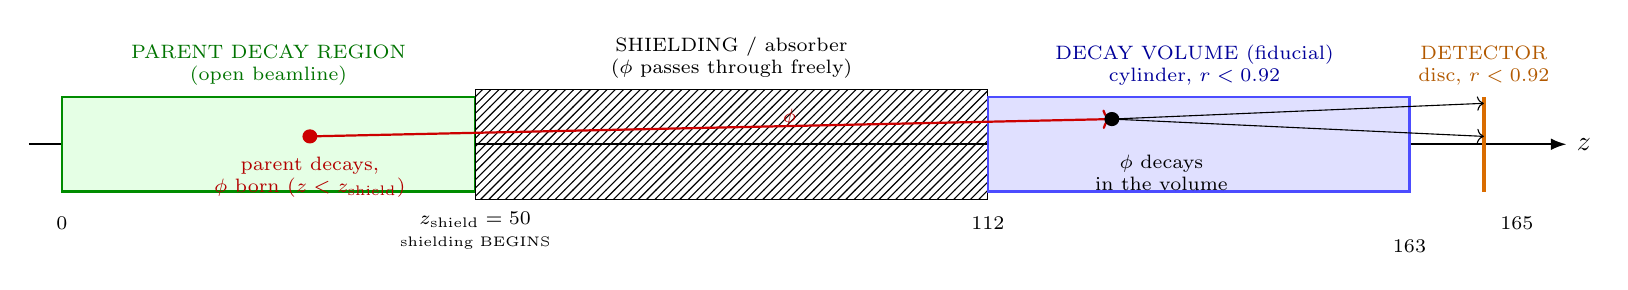
\begin{tikzpicture}[x=1.05mm,y=1mm]
  % beam line
  \draw[-{Latex[length=2mm]},thick] (-4,0) -- (182,0) node[right]{$z$};
  % parent decay region (OPEN -- this is where parents fly and decay)
  \draw[fill=green!10,draw=green!55!black,thick] (0,-6) rectangle (50,6);
  \node[align=center,font=\scriptsize,green!45!black] at (25,10)
       {PARENT DECAY REGION\\(open beamline)};
  \node[font=\scriptsize] at (0,-10) {$0$};
  % shielding STARTS at z_shield
  \fill[pattern=north east lines,draw=black] (50,-7) rectangle (112,7);
  \node[align=center,font=\scriptsize] at (81,11) {SHIELDING / absorber\\
       ($\phi$ passes through freely)};
  \node[font=\scriptsize,align=center] at (50,-11) {$z_{\rm shield}=50$\\
       \tiny shielding BEGINS};
  % decay volume
  \draw[fill=blue!12,draw=blue!70,thick] (112,-6) rectangle (163,6);
  \node[align=center,font=\scriptsize,blue!60!black] at (137,10)
       {DECAY VOLUME (fiducial)\\cylinder, $r<0.92$};
  \node[font=\scriptsize] at (112,-10) {$112$};
  \node[font=\scriptsize] at (163,-13) {$163$};
  % detector disc
  \draw[very thick,orange!85!black] (172,-6) -- (172,6);
  \node[align=center,font=\scriptsize,orange!70!black] at (172,10)
       {DETECTOR\\disc, $r<0.92$};
  \node[font=\scriptsize] at (176,-10) {$165$};
  % a phi: born INSIDE the decay region, before the shielding
  \fill[red!80!black] (30,1.0) circle (0.9);
  \node[font=\scriptsize,red!70!black,align=center] at (30,-4.2)
       {parent decays,\\$\phi$ born ($z<z_{\rm shield}$)};
  \draw[->,red!80!black,thick] (30,1.0) -- (127,3.2);
  \node[font=\scriptsize,red!70!black] at (88,3.4) {$\phi$};
  \fill (127,3.2) circle (0.9);
  \node[font=\scriptsize,align=center] at (133,-3.6) {$\phi$ decays\\in the volume};
  \draw[->,black] (127,3.2) -- (172,5.2);
  \draw[->,black] (127,3.2) -- (172,1.0);
\end{tikzpicture}
\end{center}

\paragraph{The decay volume is a fiducial region, not a detector.} A cylinder
about the beam line, $z\in[112,163]$~m, radius $0.92$~m. Nothing is measured
here; it is simply where the $\phi$ must decay for the event to count.

\paragraph{The detector is a flat disc} at $z_{\rm det}=165$~m of radius
$0.92$~m --- two metres past the downstream face of the cylinder, with the same
radius. This is what the \emph{daughters} must hit. It is a plane: no depth, no
segmentation, no efficiency, no energy threshold, no timing.

\paragraph{The shielding BEGINS at $z_{\rm shield}=50$~m.} The region
$[0,z_{\rm shield}]$ upstream of it is the open \emph{parent decay region}:
parents fly and decay there. From $z_{\rm shield}$ onward the absorber stops
everything of the Standard Model, so a parent decaying inside it produces
nothing that reaches the detector. Hence the condition is
$z_0<z_{\rm shield}$ on the $\phi$'s \emph{production} vertex --- the parent
must have decayed \emph{before} the shielding starts.

The $\phi$ itself is weakly coupled and passes through the absorber freely; the
model does not track what fills $[z_{\rm shield},z_{\min}]$, only that the
$\phi$ propagates through it undisturbed. That stretch is what gives the $\phi$
a minimum survival distance of $\gtrsim60$~m before it can be seen, and it is
what bounds the strong-coupling edge of the reach (\S\ref{sec:fates}): make
$c\tau$ short enough and the $\phi$ dies inside the absorber.

\section{What counts as a signal event}

Five conditions, applied in this order.

\begin{enumerate}
\item The $\phi$ is forward-going, $u_z>0$.
\item Its production vertex is upstream of the shielding,
  $z_0<z_{\rm shield}$ --- i.e.\ the parent decayed in the open region before
  the absorber begins.
\item Its straight-line ray intersects the cylinder. Intersecting the ray with
  the radius and the $z$-window gives the path lengths $[L_1,L_2]$ over which
  the $\phi$ is inside, \emph{measured from the production vertex}. Note $L_1$
  is where the $\phi$ \textbf{enters the volume}, not where it is born: it
  travels $0\to L_1$ through the absorber first.
\item It decays at some path length $s\in[L_1,L_2]$, i.e.\ inside the volume.
\item Its daughters reach the disc.
\end{enumerate}

\noindent Conditions 1--3 and 5 are geometry and are evaluated once. Condition
4 carries all of the coupling dependence.

\subsection{Acceptance definitions}

\paragraph{Dimuon.} Sample one isotropic $\phi\to\mu^+\mu^-$ decay, boost both
muons to the laboratory frame, propagate each in a straight line from the decay
point to $z_{\rm det}$, and require \emph{both} to be forward-going and to land
within $r_{\rm det}$. Straight lines: no magnetic field, no material, no
multiple scattering.

\paragraph{Diphoton.} For a light, highly boosted $\phi$ the two photons are
collinear with it, so the two-photon test collapses to one: continue the
$\phi$'s own line of flight from the decay point and require it to reach the
disc within $r_{\rm det}$.

\subsection{The cut flow}

Weighted, as a fraction of all $\phi$ produced:

\begin{center}
\begin{tabular}{lrr}
\toprule
 & $\mu\mu$, $\mphi=0.23$ & $\gamma\gamma$, $\mphi=0.06$ \\ \midrule
forward-going                     & 99.9996\% & 99.971\% \\
\quad + produced before the shield & 99.9996\% & 99.971\% \\
\quad + ray crosses the volume     & 15.76\%   & 12.39\%  \\
\quad + daughters hit the disc     & \textbf{8.81\%} & \textbf{7.50\%} \\
\bottomrule
\end{tabular}
\end{center}

\noindent Solid angle costs about $85\%$ at the third step. The fourth step
then removes a further $\sim40\%$, which is worth understanding: the disc has
the \emph{same} radius as the cylinder and sits only two metres beyond it, so
one might expect anything that crossed the volume to hit it. It need not. A
$\phi$ can enter near the upstream face and leave through the cylinder's
\emph{side wall} before $z_{\max}$, then continue outward and miss the disc
entirely. ``Crossed the volume'' and ``points at the detector'' are genuinely
different conditions.

\section{The decay probability is exact}
\label{sec:fates}

Given $[L_1,L_2]$ and a lab decay length $\lambda=\beta\gamma\,c\tau(g)$, the
probability of decaying inside the volume is closed-form,
\begin{equation}
  \Pdec = e^{-L_1/\lambda}-e^{-L_2/\lambda},
  \label{eq:pdec}
\end{equation}
survival \emph{to} the entrance minus survival \emph{past} the exit. A $\phi$
that decays before $L_1$ died inside the absorber or the run-up to the
volume; one that survives past $L_2$
flew through. Both are correctly and exactly excluded --- no approximation
enters here, and this is where all the $g$-dependence of the yield lives, since
$c\tau\propto g^{-2}$.

\begin{figure}[htbp]\centering
  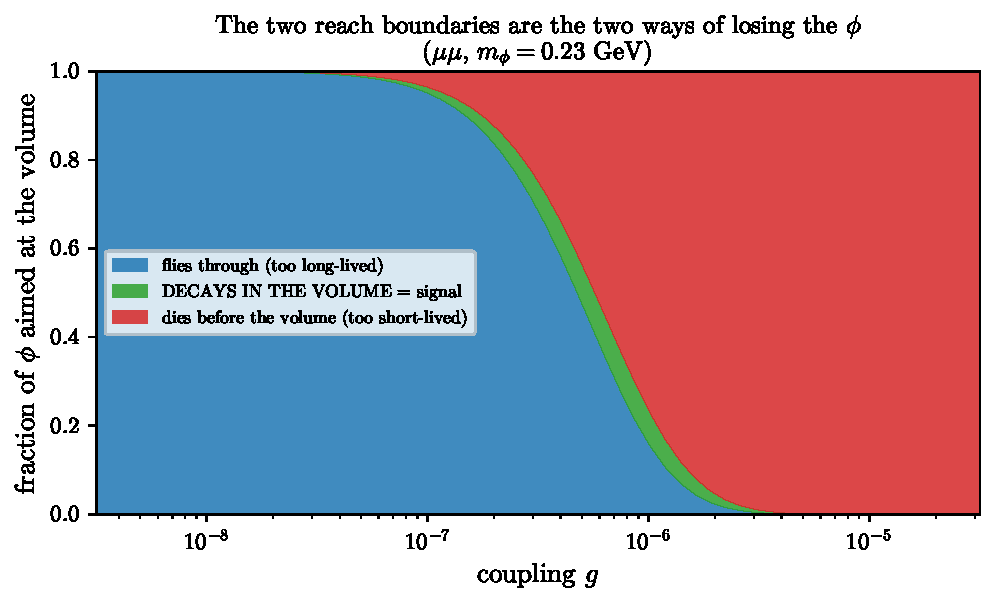
\includegraphics[width=0.72\textwidth]{figures/three_fates.pdf}
  \caption{The two reach boundaries are simply the two ways of losing the
  $\phi$. At weak coupling it is too long-lived and flies through; at strong
  coupling it is too short-lived and dies inside the absorber before
  arriving. The
  signal fraction peaks at about $8\%$ in between.}
  \label{fig:fates}
\end{figure}

\section{The approximations}

\subsection{The midpoint convention}

The acceptance depends on \emph{where} in $[L_1,L_2]$ the decay happened: decay
just inside the entrance and the muons have $\sim50$~m to spread apart and miss
the disc; decay near the exit and they have $\sim2$~m. Write that acceptance
$A(s)$. The exact contribution of one $\phi$ is
\begin{equation}
  w\int_{L_1}^{L_2}\frac{ds}{\lambda}\,e^{-s/\lambda}\,A(s),
\end{equation}
and the reference replaces it with a product,
\begin{equation}
  w\,\underbrace{\left[e^{-L_1/\lambda}-e^{-L_2/\lambda}\right]}_{\Pdec\ \text{(exact)}}
  \times
  \underbrace{A\!\left(\tfrac{L_1+L_2}{2}\right)}_{\text{acceptance at ONE fixed point}} .
  \label{eq:midpoint}
\end{equation}

\noindent In words: \emph{compute exactly the probability that it decayed
somewhere in the cylinder, then evaluate the acceptance as though every decay
occurred at the geometric centre of the cylinder crossing.}

The midpoint is taken in all three coordinates, not just in $z$:
\begin{equation}
  \mathbf{x}_{\rm mid}=\mathbf{v}+\tfrac{L_1+L_2}{2}\,\mathbf{u},
\end{equation}
with $\mathbf{v}$ the production vertex and $\mathbf{u}$ the $\phi$ direction.
That matters, because the $\phi$ walks transversely as it crosses: the median
radius runs $0.380$~m at the entrance, $0.467$~m at the midpoint and $0.555$~m
at the exit --- a $0.134$~m walk against a $0.92$~m volume radius, so $15\%$ of
the aperture. The daughters are therefore launched from a point displaced
radially by up to $\pm0.07$~m from where the decay really happened, as well as
from the wrong $z$.

\paragraph{For $\gamma\gamma$ this is not an approximation at all.} The photons
are collinear with the $\phi$, so they continue along the \emph{same line}, and
the dependence on $s$ cancels identically. Writing the transverse landing point
on the disc,
\begin{equation}
  \mathbf{x}^{\rm land}_\perp
  =\underbrace{\mathbf{v}_\perp+s\,\mathbf{u}_\perp}_{\text{decay point}}
  +\underbrace{\left[\frac{z_{\rm det}-v_z}{u_z}-s\right]\mathbf{u}_\perp}
              _{\text{flight to the disc}}
  =\mathbf{v}_\perp+\frac{z_{\rm det}-v_z}{u_z}\,\mathbf{u}_\perp ,
  \label{eq:photon_cancel}
\end{equation}
independent of $s$: moving the decay point along the line trades transverse
displacement against remaining lever arm in exactly compensating amounts.
Numerically the landing radius at the entrance and at the exit differ by
$9\times10^{-16}$~m, i.e.\ machine epsilon. So the flatness of the
$\gamma\gamma$ curve in \cref{fig:acc} is an algebraic identity, not a good
approximation, and the midpoint convention introduces \emph{no} error in the
diphoton channel.

\paragraph{For $\mu\mu$ the cancellation is incomplete.} Each muon leaves along
its own direction $\mathbf{k}$ rather than $\mathbf{u}$, so the flight term in
\cref{eq:photon_cancel} carries $\mathbf{k}_\perp/k_z$ while the displacement
term still carries $\mathbf{u}_\perp$. The two no longer cancel, and both the
residual transverse offset and the changed lever arm survive. That is the
entire origin of the variation measured below.

\paragraph{Why.} $A(\text{midpoint})$ does not depend on $g$, so one
precomputed sample serves the entire coupling axis: $L_1$, $L_2$,
$\beta\gamma$, the weights and $A$ are computed once, and
\cref{eq:pdec} then supplies every coupling analytically. A 400-point scan
costs one flux and carries no additional Monte-Carlo noise. Sampling the true
decay point instead would make $A$ depend on $g$, forcing a fresh sample at
every coupling and injecting scatter into the reach contour --- on the branch
where scatter hurts most.

\paragraph{What it costs.} \Cref{fig:acc} shows $A(s)$ measured across the
crossing. For $\mu\mu$ it rises from $0.508$ at the entrance to $0.625$ at the
exit, a $23\%$ swing, with the midpoint at $0.559$. For $\gamma\gamma$ it is
flat at $0.60514$ to five digits, for the reason just given.

\begin{figure}[htbp]\centering
  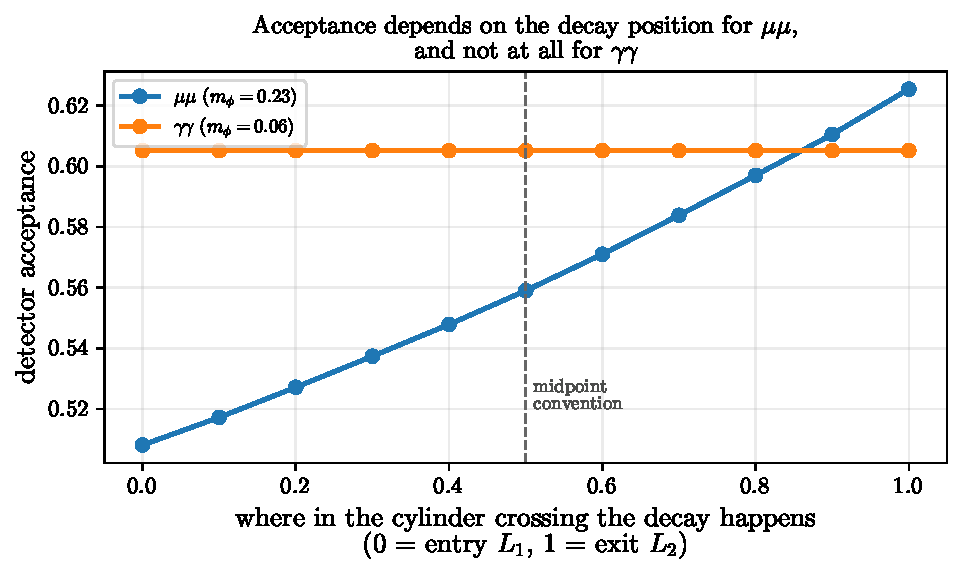
\includegraphics[width=0.7\textwidth]{figures/acceptance_vs_position.pdf}
  \caption{Acceptance against where in the cylinder crossing the decay occurs.}
  \label{fig:acc}
\end{figure}

A $23\%$ swing sounds serious, and one would expect the approximation to fail
at strong coupling, where $\lambda$ shrinks and decays pile up near the
entrance. It does not --- the error \emph{falls}:

\begin{center}
\begin{tabular}{rrrr}
\toprule
$g$ & median $\lambda$ & yield-weighted $\lambda$ & error [dex] \\ \midrule
$1\times10^{-6}$ & 147~m & 116~m & 0.0029 \\
$3\times10^{-6}$ & 16.4~m & 54.7~m & 0.0002 \\
$6\times10^{-6}$ & 4.1~m & 36.0~m & 0.0000 \\
$1\times10^{-5}$ & 1.5~m & 24.1~m & 0.0000 \\
\bottomrule
\end{tabular}
\end{center}

\noindent The reason is a selection effect. $\Pdec\sim e^{-L_1/\lambda}$
suppresses short-$\lambda$ events astronomically --- at $\lambda=4$~m against
$L_1=112$~m that is $e^{-28}$ --- so whatever the median $\phi$ is doing, the
ones that actually contribute are always the long-lived tail, whose decays
remain spread across the cylinder. The weighting selects precisely the
population for which the midpoint is a good centre.

\paragraph{Verdict.} $\leq0.004$~dex for $\mu\mu$, identically zero for
$\gamma\gamma$. For scale, the best unaided agents in the 2026-08 campaign sit
at $0.017$~dex, so this is a quarter of the smallest error currently
resolvable. An agent that samples the true decay point will be \emph{more}
correct than the reference, by an amount below the noise floor.

\subsection{The forward harvest cone $\theta_{\max}$}

Parents are harvested from the generator only within $\theta<\theta_{\max}$ of
the beam axis; the reference uses $\theta_{\max}=0.05$~rad. This is a
pre-filter to bound the flux file, and it is the one ``obvious'' parameter with
a wrong-but-reasonable answer sitting next to it.

The naive sizing is that the volume subtends $r/z=0.92/112=8.2$~mrad, so
$\sim10$~mrad ought to be ample. It is not, because the $\phi$ is \emph{not}
collinear with its parent: it is emitted with rest-frame momentum $p^\star$,
giving $\Delta\theta\sim p^\star/E$. A parent outside the geometric cone can
still emit a $\phi$ into it. (The median parent sits at $2.7$~mrad while the
median $\phi$ sits at $3.6$~mrad --- the daughter is at \emph{larger} angle.)

\begin{figure}[htbp]\centering
  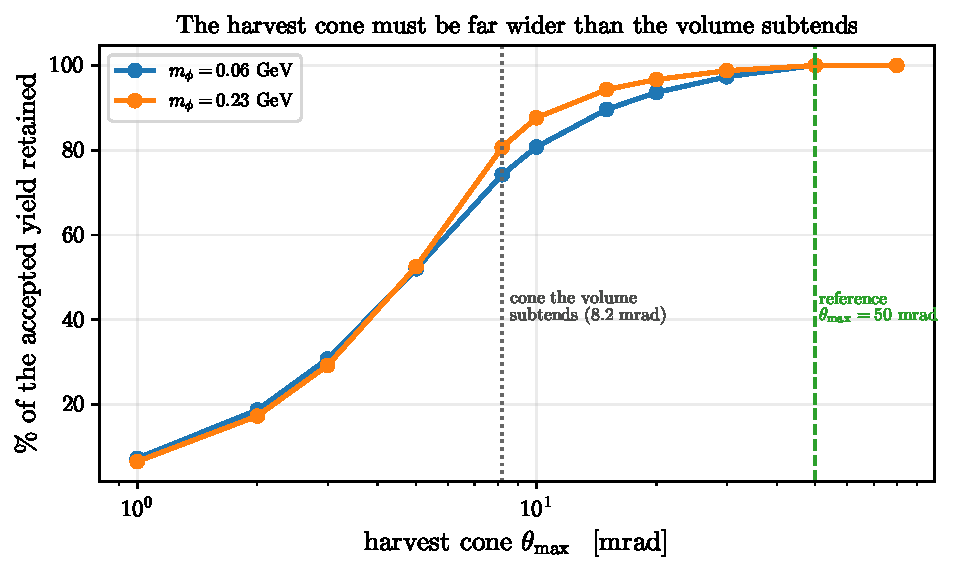
\includegraphics[width=0.7\textwidth]{figures/theta_max.pdf}
  \caption{Fraction of the accepted yield retained as a function of the harvest
  cone. Cutting at the cone the volume subtends keeps only $\sim74\%$.}
  \label{fig:theta}
\end{figure}

\noindent Cutting at $8.2$~mrad retains $73.9\%$; at $10$~mrad, $80.4\%$; at
$20$~mrad, $93.5\%$; at $50$~mrad, $100.000\%$. So $\theta_{\max}=0.05$~rad is a
deliberate $\sim6\times$ over-harvest, and the plausible choice of $10$~mrad
silently loses $20\%$ --- $0.1$~dex, six times the best agent's error.
\textbf{This is a pin, not a free parameter.}

\subsection{Stratified decay-length sampling}

The parent decay length is drawn by splitting its exponential into $K$
equal-probability strata and taking one point at random inside each. Until
2.5.0 the point was the stratum \emph{midpoint}, which is a quadrature rule
rather than stratified sampling and carries $O(1)$ error when a discontinuity
falls inside a panel --- and the $z_{\rm shield}$ cut is exactly such a
discontinuity. At $K=6$ the yield was low by five orders of magnitude near the
strong-coupling edge, identically for every seed. Randomising within the
stratum removes the bias at any $K$. See
\texttt{benchmarks/llp_forward/soln/notes/strata\_convergence.md}.

\subsection{The hemisphere fold (a bug, now fixed)}

The forward cut is taken about the beam \emph{axis}, so both cones are
harvested and stored with $p_z\to|p_z|$. That doubles the sample and therefore
requires halving the per-collision weight. The factor was missing, so every
flux --- and every yield built on one --- was $2\times$ too large. The detector
is single-arm, so a genuinely backward parent can never reach it: folding is
variance reduction, not extra flux. Fixed 2026-08-08; the reference has been
regenerated.

\section{Summary of approximations}

\begin{center}
\begin{tabular}{lll}
\toprule
& status & measured cost \\ \midrule
$\Pdec$ (\cref{eq:pdec})           & exact & --- \\
midpoint acceptance                & approximation ($\mu\mu$ only) & $\leq0.004$~dex; EXACT for $\gamma\gamma$ \\
$\theta_{\max}=0.05$~rad           & pin & $0$ at this value; $0.1$~dex at 10~mrad \\
stratified decay length            & fixed in 2.5.0 & was 5 orders of magnitude at $K=6$ \\
hemisphere fold                    & bug, fixed & was exactly $2\times$ \\
straight-line daughters            & modelling & no field/material/scattering \\
disc detector                      & modelling & no efficiency, resolution or background \\
\bottomrule
\end{tabular}
\end{center}

\vspace{1em}
\noindent\rule{\textwidth}{0.4pt}\\[0.3em]
{\small Figures and every number quoted here are produced by
\texttt{lib/make\_detector\_figures.py} in \texttt{hepbench-analysis} from the shipped
implementation and the archived flux.}

\end{document}
